\documentclass[12pt]{article}
\usepackage{graphicx}
\usepackage{subfig}
\usepackage{float}
\usepackage[margin=1in,includefoot]{geometry}
\usepackage{fancyhdr}
\pagestyle{fancy}
\renewcommand{\footrulewidth}{1pt}

\begin{document}

\begin{titlepage}
	\begin{center}
	\begin{figure}[t]
	\hspace*{0.35cm}
\includegraphics[width=1.0\textwidth]{uclLogo}\\
	\end{figure}
	\line(1,0){300}\\
	[0.25in]
	\huge{\bfseries ArcheoReport}\\
	[2mm]
	\line(1,0){200}\\
	[1.5cm]
	\textsc{\LARGE University College London}\\
	\textsc{\normalsize Department of Computer Science}\\
	\textsc{\normalsize COMP103P Application Project}\\
	\textsc{\normalsize Team38}\\
	[5cm]
	\end{center}
	\begin{flushright}
	{\large Authors: \\}
	Mohammad Hossein Afsharmoqaddam\\
	Varun Mathur
	\end{flushright}
\end{titlepage}
\tableofcontents

\newpage
\section{Abstract}\label{sec:abstract}
Our application project was assigned to the Egyptian Museum of Turin, Italy. We had to develop an exhibition based management tool which would be used by the museum professionals when they are hosting exhibitions outside of their local location. It is essentially an effective tool for museums with archaeological collections.  
\par
The application is designed in such a way where the user is able to create a full ``condition report''  about the state of preservation of the artefacts. ``A condition report'' is a detailed description of the condition of a museum artefact typically produced on the occasion of loans for exhibitions, special handling sessions, packing or restoration projects. 
\par
Additionally, the user is then able to generate a pdf file after filling out the form and save it to their database for further references and creating new forms. To expand, the app has a simple and user friendly interface with various field and dropdown menus and controlled vocabularies and it is able to acquire multiple images of the artefacts. The application allows the user to either upload a photo from the directory of their device or to take a photo from the camera provided on their device. After uploading the photo they are able to annotate the photos using their fingers or a tablet pen. 
\par
Furthermore, the application provides two view screens which are, the ``view forms'' and ``view gallery''. Both of these screens showcase and group their data and the user is able to filter the data by the filtering options provided. 




\newpage
\section{Context}\label{sec:context}

\subsection{Background}
Our team has been in contact with Paolo Del Vesco, a UCL honorary researcher and a curator at the museum and Marco Rossani the registrar of the museum.  The Egyptian Museum of Turin also known as ``Museo delle Antichita'' is the only museum other than the Cairo museum that is dedicated solely to Egyptian art and culture. According to the museums website ``the collections that make up today’s Museum were enlarged by the excavations conducted in Egypt by the Museum’s archaeological mission between 1900 and 1935 (a period when finds were divided between the excavators and Egypt).''

\subsection{Purpose}\label{sec:purpose}
As discussed in the Abstract the museum loans artefacts for exhibitions, have special handling sessions and packing or restoration projects. Therefore, the museum needs to be able to keep track of each artefact and be able to check the artefacts conditions before and after the sessions. 
\par
However, majority of these actions have been paper form based and this application fundamentally will be digitalising the records of the artefacts. By digitalising the system we have brought many advantages which were not possible before in the paper based system which will be discussed below.  

\subsubsection{Easy Access}
From the moment a form is created it becomes accessible from any of the tablets which has the application downloaded. By having a paper based system, a paper file cannot be accessing by another employee at the same time and it is usually housed in file or cabinet which access must be requested.

\subsubsection{Filtering and Searchable Text}
The application allows the user to be able to locate and view forms based on their specific exhibition date and also has a gallery screen which provides all of the photos of the artefacts which can be filtered by the different parameters provided. This is extremely useful since if a client request a form, the museum will be able easily search the form required from their database.

\subsubsection{Cost Savings}
The switch to digitalising a system saves money for many establishments. By having a digitalised system we are minimising the cost of papers, secure file cabinets that the files need to be archived in and adding this to the cost of filing clerks and the downtime required to find specific forms the cost increases substantially.



\newpage
\section{Team Member Summary}

\subsection{Mohammad Hossein Afsharmoqaddam}
Mo did not have any prior android development experience, therefore this was a new area for him to explore. He previously has had experience with C and Java from his university courses and basic web development. He has always liked frontend development and design, therefore his responsibilities were mainly the User Interface elements, navigation and the overall Logic of the application. 

\subsection{Varun Mathur}


\subsection{Rouzbeh Mehregan}





\newpage
\section{Work Plan (GANTT CHART)}
To be as efficient and productive as possible and a Gantt Chart offers many advantages we decided to use this method to enhance our communication, and to be able to see our project over the long term and to track the results of each task. 
\par
In a glance we were able to keep track of incoming tasks, and tasks that remained to be completed, therefore we avoided any completion confusion. Furthermore, by being able to look ahead we were able to effectively allocate resources and tasks to each member. 

\begin{figure}[h]
\begin{center}
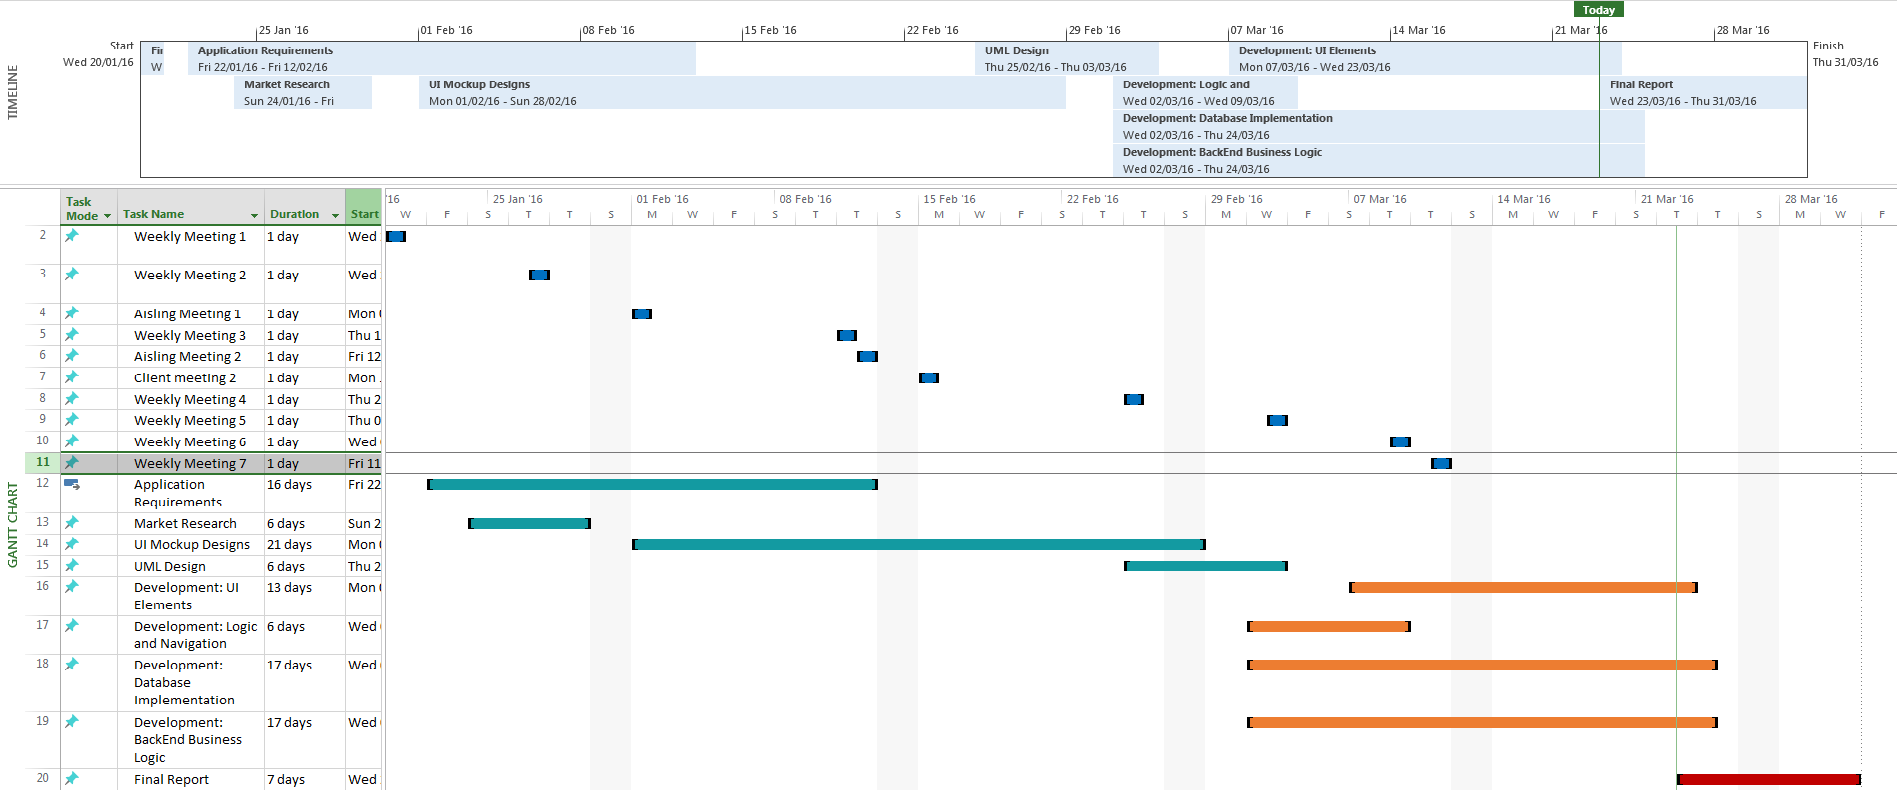
\includegraphics[width=1.0\textwidth]{ArcheoReportGantt}
\end{center}
\end{figure}

As you can see from the figure, we separated the project into three different areas. The blue colour reprsents our team meetings during the project, the turquoise colour represents the timeline of our early planning, requirements and mock-up stages. The orange colour represents our development and programming phase and the red colour represents the evaluation and the creation of the final report. Additionally, the timeline on top of the chart provides us with the exact duration that each task should be completed. 
\end{document}
